\documentclass{article}

\usepackage{amssymb,amsmath}
\numberwithin{equation}{section}
\usepackage{dcolumn}% Align table columns on decimal point
\usepackage{bm}% bold math
\usepackage[utf8]{inputenc}
\usepackage[spanish,es-tabla]{babel}
\usepackage{hyperref}
\hypersetup{
    colorlinks=true,
    linkcolor=blue,
    urlcolor=red,
    linktoc=all
}
\usepackage[left=3cm,top=2.5cm,right=3cm,bottom =2.5cm,nohead,nofoot]{geometry}

\usepackage{enumerate}
\usepackage{graphicx}

\usepackage{amsthm}

\newtheorem{theorem}{Teorema}[section]

\theoremstyle{definition}
\newtheorem{definition}{Definición}[section]


\begin{document}

\begin{titlepage}
	\centering
	\vspace*{\baselineskip} 
	
\includegraphics[width=0.5\textwidth]{logo_uniandes}\par\vspace{1cm}
%	{\scshape\LARGE Universidad de Los Andes \par}
%	\vspace{1cm}
	{\scshape\Large Proyecto de Grado en Física\par}
	\vspace{1.5cm}
	\rule{\textwidth}{1.6pt}\vspace*{-\baselineskip}\vspace*{2pt}
	\rule{\textwidth}{0.4pt}\\[\baselineskip]
	{\huge\bfseries Estudio de estrellas de Planck\par}
	\rule{\textwidth}{0.4pt}\vspace*{-\baselineskip}\vspace{3.2pt}
	\rule{\textwidth}{1.6pt}\\[\baselineskip]
	\vspace{2cm}
	{\Large\itshape Alejandro Hernández A.\par}
	\vfill
	Director:\par
	Dr. Pedro Bargueño de Retes 
	\vfill

% Bottom of the page
	{\large 9 de Marzo de 2016\par}
\end{titlepage}

\newpage
\large
\tableofcontents
\newpage

\normalsize
\section{Introducción}

Desde la publicación del famoso artículo \textit{The Foundation of the General Theory of Relativity} %\cite{einstein} 
por Albert Einstein en el año de 1916, la búsqueda de soluciones exactas a sus ecuaciones de campo ha sido uno de los principales motores de investigación en relatividad general (GR). La primera solución matemática exacta de dichas ecuaciones fue la métrica de Schwarzschild, que describe la geometría generada en el exterior de un cuerpo esféricamente simétrico, sin carga y sin momento angular. Además de la anterior, otra métrica que presenta simetría esférica es la de Reissner Nordström (métrica RN), la cual describe un cuerpo cargado sin rotación. Estas métricas comparten una característica particular, a saber, ambas poseen una singularidad física en $r = 0$. Esto dificulta el tratamiento de ese punto tanto en el espaciotiempo de Schwarzschild como en el de Reissner Norström, puesto que la teoría no es aplicable en el susodicho punto singular.\\

Teniendo en cuenta lo anterior, los puntos singulares de un espaciotiempo dado dejan entrever fallas de la teoría general de la relatividad puesto que no permite describir las propiedades físicas de los mismos. Con el fin de evadir estas dificultades, se dice que un agujero es regular, o sin puntos singulares, cuando los invariantes de curvatura $R$, $R^{\mu \nu}R_{\mu \nu}$, $R^{\mu \nu \rho \sigma}R_{\mu \nu \rho \sigma}$ son finitos en todos los puntos del espaciotiempo en cuestion. Dado esto, desde hace más de cincuenta años el estudio de espaciotiempos (agujeros negros) regulares ha sido de gran interés para múltiples físicos y matemáticos, entre ellos, James M. Bardeen. \\

En el año de 1968, Bardeen fue el primero en proponer una solución regular de las ecuaciones de campo de Einstein. Si bien el documento \cite{bardeen} en el que se propuso el modelo no está disponible, una revisión detallada de la métrica de Bardeen puede ser consultada en \cite{borde1994}. La importancia de esta métrica no solo se debe a que fue la primera de su estilo sino también a que fue crucial para orientar las futuras investigaciones sobre agujeros negros regulares. Al respecto, Ayón-Beato y García propusieron una interpretación física del modelo de Bardeen en términos de electrodinámica no lineal  \cite{ayon-beato2000} y construyeron muchos otras métricas correspondientes a agujeros negros regulares \cite{ayon-beato2005,ayon-beato1999-1,ayon-beato1999-2,ayon-beato1999-3}.\\

Ayende de lo anterior, trabajos más recientes \cite{hayward2006,lorenzo,rovelli} tratan de generalizar el modelo que propuso Bardeen de regularización de agujeros negros, de tal forma que se incluyan correcciones efectivas de teoría cuántica de campos en relatividad general. En estos modelos se definen el concepto de Estrella de Planck, que corresponde a un métrica regular, esféricamente simétrica, asintóticamente plana, que satisface la condición de energía débil y que no posee horizontes de Cauchy (¡OJO!).\\

Precisamente, el objetivo de este trabajo es entender el proceso mediante el cual se formulan las métricas correspondientes a estrellas de Planck, entender el mecanismo mediante el cual dichas métrica evaden la singularidad en $r = 0$ (¡OJO!), además de tratar de interpretar físicamente el tensor de energía-momento (SET) asociado a las mismas. Teniendo en cuenta lo previamente mencionado, la organización de este documento se da a continuación. En la Sec. \ref{preliminaries section} se establecen las condiciones de energía de forma usual en términos de SET y se establece la metodología general que se empleará para estudiar todas las métricas presentadas. En la Sec. \ref{previous metrics section} se estudian en detalle las métricas de Bardeen y de Vaidya, las cuales constituyen la base sobre la cual se definen las estrellas de Planck. Posteriormente, en la Sec. \ref{planck stars section} se estudia a fondo la métrica que define las aludidas estrellas de Planck y se da la interpretación física de las mismas. Finalmente, en la sección \ref{conclusions} se resumen los resultados del trabajo y en la sección \ref{annex} se habla sobre las correcciones cuánticas que introducen las estrellas de Planck en relatividad general.\\

¡OJO! Teoremas de singularidad.

\section{\label{preliminaries section} Preliminares}

%¡OJO! Ejemplos cuando se hable de cada métrica.\\
%¡OJO! Blau Notes \\
%
%Existen diversos tipos de horizontes en relatividad general y las definiciones dadas en esta sección solo se remiten a aquellos horizontes que serán utilizados en el estudio posterior de las diversas métricas que se presentarán posteriormente.
%
%\subsection{Horizontes de eventos}
%
%Un horizonte de eventos es una frontera en el espacio-tiempo más allá de la cual los eventos que ocurran en su interior no pueden afectar a un observador externo. Para el caso particular de los agujeros negros, un horizonte de eventos puede ser entendido como la forntera a partir de la cual la velocidad necesaria para escapar del campo gravitacional del agujaro supera la velocidad de la luz.\\
%
%Dada una métrica en coordenadas esféricas $(t,r,\theta,\phi)$, los horizontes de eventos de dicha métrica se localizan en los puntos donde $g^{rr}$ diverge.
%
%\subsection{Horizontes de Killing}
%
%Antes de definir un horizonte de Killing es preciso definir vectores de killing. Un campo vectorial de killing $X$ es, valga la redundancia, un campo vectorial que satisface
%
%\begin{equation}
%\nabla_\mu X_\nu + \nabla_\nu X_\mu = 0,
%\end{equation}
%
%es decir, que la derivada covvariante de este campo vectorial es antisimétrica (¡OJO!). Teniendo en cuenta lo anterior, un horizonte de killing se define como una hipersuperficie nula donde la norma de un vector de killing se hace cero.
%
%\subsection{Horizontes aparentes}
%
%Los horizontes aparentes son \cite{blau}.

	\subsection{Condiciones de energía}

De vital importancia para el estudio de las métricas a lo largo de todo este documento son las denominadas condiciones de energía. Si bien en la mayoría de los casos resulta útil estudiar las ecuaciones de campo sin especificar la fuente de materia $T_{\mu \nu}$ en el espacio-tiempo descrito, en algunas ocasiones resulta interesante estudiar las propiedades de dichas ecuaciones que son válidas para diversas fuentes de materia. En esta última situación es fundamental imponer condiciones de energía que limiten la arbitrariedad de $T_{\mu \nu}$ con el fin de que sean fuentes razonables de energía y momento \cite{carroll}.\\

Las formulaciones matemáticas de las múltiples  condiciones de energía se establecen a continuación:

\begin{itemize}
\item \textbf{Condición de energía débil (WEC):} Para todo vector timelike $t^\mu$ se satisface $T_{\mu \nu}t^{\mu}t^{\nu} \geq 0$. Para el caso particular de un fluido perfecto esta condición se traduce en $\rho \geq 0$ y $\rho + p \geq 0$.

\item \textbf{Condición de energía débil (NEC):} Como caso expecial de WEC, se exige que para cualquier vector nulo $l^\mu$ se tenga $T_{\mu \nu}l^{\mu}l^{\nu} \geq 0$. En el caso de un fluido perfecto, esta condición exige $\rho + p \geq 0$.

\item \textbf{Condición de energía dominante (DEC):} Esta condición incluye a WEC y se puede dividir en dos partes: la primera es exactamente igual a lo requerido por WEC; y la segunda exige que $T_{\mu \nu}T^{\nu}_{\ \lambda}t^{\mu}t^{\lambda} \geq 0$ para todo $t^{\mu}$ timelike. Para fluidos perfectos esta condición se traduce en $\rho \geq |p|$.

\item \textbf{Condición de energía fuerte (SEC):} Esta última condición exige que $T_{\mu \nu}t^{\mu}t^{\nu} \geq \frac{1}{2}T^{\lambda}_{\ \lambda}t^{\sigma}t_{\sigma}$ para todo vector $t^\mu$ timelike. Equivalentemente, se demanda que $\rho + p \geq 0$ y que $\rho + 3p \geq 0$ en el caso de un fluido perfecto. Cabe mencionar que la SEC no implica a WEC pero sí implica a NEC.
\end{itemize}

Como se verá más adelante, las únicas dos condiciones de energía que realmente interesan para el estudio de agujeros negros regulares son la WEC y la SEC, esto por el significado físico que hay destrás de estas condiciones, a saber, la WEC establece la no-negatividad de la densidad de energía para cualquier observador, mientras que la SEC alude al carácter atractivo de la fuerza gravitatoria.\\

\subsection{Procedimiento General}

Teniendo en cuenta el Teorema de Birkhoff \cite{gravitation} y la derivación hecha en \cite[Cap. 7]{carroll-lecture-notes} de la métrica de Schwarzschild, la forma más general de una métrica estática y esféricamente simétrica es

\begin{equation}
\label{general static spherical}
ds^2 = -f(r)dt^2 + \frac{1}{f(r)}dr^2 + r^2d\Omega^2,
\end{equation}

donde la función $f(r)$ puede ser escrita como

\begin{equation}
\label{general f}
f(r) = 1 - \frac{2m(r)}{r}.
\end{equation}

Ahora bien, dado que nos interesa estudiar agujeros negros regulares, es preciso aclarar que la SEC se debe violar en algún lugar dentro del horizonte \cite{zaslavskii}, a la vez que la WEC o la DEC pueden ser satisfechas en todo el espaciotiempo generado \cite{dymnikova2004}. Al considerar el elemento de línea \eqref{general static spherical} junto con \eqref{general f}, es posbile escribir los componente de SET como \cite{vanegas-weak} OJO signatura y métrica ortogonal

\begin{equation}
\label{wec set comp}
\begin{aligned}
T^{t}_{\ t} = T^{r}_{\ r} = \frac{2}{8 \pi r^2} \frac{dm(r)}{dr},\\ T{^\theta}_{\theta} = T^{\phi}_{\ \phi} = \frac{1}{8 \pi r} \frac{d^2m(r)}{dr^2},
\end{aligned}
\end{equation}

y por ende, se concluye que la WEC puede expresarse de manera equivalente en términos de la función de masa $m(r)$ mediante las siguientes desigualdades

\begin{equation}
\label{mass wec ineq}
\begin{aligned}
\frac{1}{r^2}\frac{dm(r)}{dr} &\geq 0,\\
\frac{2}{r}\frac{dm(r)}{dr} &\geq \frac{d^2m(r)}{dr^2}.
\end{aligned}
\end{equation}

Como se mencionó previamente, la DEC incluye por continuidad a la WEC. Esto permite argumentar que, por simplicidad, la única condición de energía que se va a exigir para los agujeros negros regulares presentados en secciones poseriores será la WEC.

\section{\label{previous metrics section} Métricas relevantes}

A continuación se realiza un estudio detallado de las métricas de Bardeen y de Vaidya, las cuales son cruciales para el estudio posterior de la métrica que describe el espaciotiempo generado por las estrellas de Planck.

\subsection{\label{bardeen section} Métrica de Bardeen}

Como se mencionó en la introducción, la métrica de Bardeen \cite{bardeen} fue la primera en describir un espaciotiempo regular. En coordenadas esféricas $(t,r,\theta,\phi)$, la métrica de Bardeen se expresa como

\begin{equation}
\label{bardeen metric}
ds^2 = -\left( 1 - \frac{2mr^2}{(r^2 + g^2)^{3/2}} \right)dt^2 + \left( 1 - \frac{2mr^2}{(r^2 + g^2)^{3/2}} \right)^{-1}dr^2 + r^2d\Omega^2,
\end{equation}

con $m$ y $q$ parámetros no negativos, en algunos casos llamados parámetros de regularización. Claramente, para esta métrica tenemos que 

\begin{equation}
m(r) = \frac{2mr^3}{(r^2 + g^2)^{3/2}},
\end{equation}

por tanto, la WEC se satisface automáticamente en cualquier punto del espacio tiempo puesto que 

\begin{align}
\begin{aligned}
\frac{1}{r^2}\frac{dm(r)}{dr} &= \frac{6 m g^2}{\left(g^2+r^2\right)^{5/2}},\\
\frac{2}{r}\frac{dm(r)}{dr} &= \frac{12 m g^2 r}{\left(g^2+r^2\right)^{5/2}},\\
\frac{d^2m(r)}{dr^2} &= \frac{6 m \left(2 g^4 r-3 g^2 r^3\right)}{\left(g^2+r^2\right)^{7/2}}.
\end{aligned}
\end{align}

El carácter regular de la métrica de Bardeen es evidente a partir del hecho de que, por un lado

\begin{equation}
f_{bardeen}(r) \underset{r \to 0}{\sim} 1 - \frac{2mr^2}{g^3} + \mathcal{O}(r^4),
\end{equation}

es decir, posee un comportamiento de de Sitter en la vecindad de $r = 0$, y por otro, los escalares de curvatura

\begin{equation}
\label{bardeen scalars}
\begin{gathered}
R = \frac{6 g^2 m \left(4 g^2-r^2\right)}{\left(g^2+r^2\right)^{7/2}},\\
R_{\mu \nu}R^{\mu \nu} = \frac{18 g^4 m^2 \left(8 g^4-4 g^2 r^2+13 r^4\right)}{\left(g^2+r^2\right)^7},\\
R_{\mu \nu \sigma \rho}R^{\mu \nu \sigma \rho} = \frac{12 m^2 \left(8 g^8-4 g^6 r^2+47 g^4 r^4-12 g^2 r^6+4 r^8\right)}{\left(g^2+r^2\right)^7},
\end{gathered}
\end{equation}

son finitos en todo punto  del espaciotiempo.\\

Ahora bien, debido a que el elemento de línea \eqref{bardeen metric} es diagonal, es posbile obtener los horizontes de eventos de esta métrica al solucionar

\begin{equation}
f_{bardeen}(r) = 1 - \frac{2mr^2}{(r^2 + g^2)^{3/2}} = 0.
\end{equation}

Y analizar las condiciones para la existencia de soluciones reales se concluye que la métrica \eqref{bardeen metric} describe un agujero negro (es decir, posee horizontes de eventos) para $g^2 \leq (16/27)m^2$: cuando $g^2 < (16/27)m^2$ existen dos horizontes de eventos $r_{+},r_{-}$ y cuando $g^2 = (16/27)m^2$ solo hay un horizonte de eventos degenerado $r_{+} = r_{-}$. En este último caso se dice que el agujero negro es extremal, tal y como en la métrica RN, en tanto que posee un único horizonte de eventos. Es importante recalcar que en cualquier caso, los horizontes de eventos para el agujero negro de Bardeen tan solo constituyen singularidades debidas al sistema de coordenadas puesto que ya se mencionó que los invariantes de curvatura (\ref{bardeen scalar}-\ref{bardeen riemann scalar}) son finitos en todo el espaciotiempo. La extensión de la métrica de Bardeen más allá de los horizontes de eventos se puede hacer al cambiar a las coordenadas de Eddington-Finkelstein salientes, en términos de las cuales la métrica es bien comportada incluso en el caso del agujero negro extremal. \\

Considere nuevamente la componente temporal $g_{tt}$ de la métrica \eqref{bardeen metric}. Note que

\begin{equation}
f_{bardeen}(r) \underset{r \to \infty}{\sim} 1 - \frac{2m}{r} + \frac{3mg^2}{r^3} + \mathcal{O}\left( \frac{1}{r^5} \right).
\end{equation}

Los dos primeros términos de la expansión corresponden, como es de esperarse, al comportamiento asintóticamente plano de la métrica de Bardeen, y por tanto, es posible identificar al parámetro $m$ como la masa de la configuración descrita por esta métrica. No obstante, el término $1/r^3$ impide asociar el parámetro  de regularización $g$ con algún tipo de carga de Coulomb, a diferencia de la métrica de Reisner Norström, en la que el parámetro $q$ es automáticamente asociado a una carga eléctrica al comparar el SET de esta métrica con el del campo eléctrico para una carga puntual. Este hecho fue el principal obstáculo para la interpretación física del parámetro $g$ en la métrica de Bardeen hasta que Ayón-Beato y García propusieron una interpretación en términos de electrodinámica no-lineal \cite{ayon-beato2000}.\\

El modelo de Ayón-Beato y García parte la suposición de que la dinámica de la métrica de Bardeen está regida por

\begin{equation}
\mathcal{S} = \int dv \left( \frac{1}{16 \pi}R - \frac{1}{4 \pi}\mathcal{L}(F) \right),
\end{equation}

donde $R$ es el escalar de curvatura; $\mathcal{L}$ es una función de $F = \frac{1}{4}F_{\mu \nu}F^{\mu \nu}$, con $F_{\mu \nu} = 2\nabla_{[\mu}A_{\nu]}$ el tensor electromagnético; y $v$ es la coordenada avanzada de Eddington-Finkelstein. Las ecuaciones de Eisntein acopladas con electrodinámica no-lineal resultantes de la acción $\mathcal{S}$ son (¡OJO!)\\

\begin{equation}
\label{euler lagrange eqns}
\begin{aligned}
G_{\mu}^{\ \nu} = 2(\mathcal{L}_{F} F_{\mu \lambda} F^{\nu \lambda} - \delta_{\mu}^{\ \nu} \mathcal{L}),\\
\nabla_{\mu}(\mathcal{L}_{F} F^{\alpha \mu}) = 0,
\end{aligned}
\end{equation}

donde $\mathcal{L}_{F} \equiv \partial \mathcal{L}/\partial F$. La fuente electrodinámica no-lineal usada por los autores para derivar la métrica de Bardeen es (¡OJO! Formalismo P)

\begin{equation}
\label{nonlinear bardeen}
\mathcal{L}(F) = \frac{3}{2sg^2}\left( \frac{\sqrt{2g^2F}}{1 + \sqrt{2g^2F}} \right)^{5/2},
\end{equation}

donde $s \equiv |g|/2m$; m la masa de la configuración descrita; y $g$ un parámetro de integración. Además, los autores consideran el ansatz para el campo electromagnético 

\begin{equation}
F_{\mu \nu} = 2 \delta^{\theta}_{\ \lbrack\mu} \delta^{\varphi}_{\ \nu\rbrack} B(r, \theta),
\end{equation}

y al tener en cuenta todas las consideraciones previamente mencionadas, Ayón-Beato y García concluyen que el parámetro $g$ corresponde a la carga de un monopolo magnético, esto es (¡OJO!)

\begin{equation}
\frac{1}{4 \pi} \int_{S^{\infty}}\mathbf{F} = \frac{g}{4 \pi} \int_{0}^{\pi}\int_{0}^{2\pi}\sin (\theta) d\theta d\varphi = g.
\end{equation}

Todo lo anterior permite entender la métrica \eqref{bardeen metric} como un acople de electrodinámica no-lineal a la relatividad general, que físicamente corresponde a un monopolo magnético autogravitante de carga $g$. Esta interpretación de la métrica de Bardeen hace eco de una de las características fundamentales de la métrica RN en tanto que las propiedades globales del espacio-tiempo descrito tanto por la métrica de Reissner-Nordström como por la métrica de Bardeen dependen fuertemente de las magnitudes relativas entre el parámetro de carga y el parámetro de masa.\\

Ahora bien, hasta el momento solo se ha lidiado con la interpretación física de la métrica de Bardeen \eqref{bardeen metric} y se ha establecido el carácter regular de la misma en términos de la finitud de los invariantes de curvatura. No obstante, es preciso ahondar un poco más en el último aspecto mencionado, dado que es el principal motivo para estudiar dicha métrica en este trabajo.\\

En el año 1965, Roger Penrose publicó un famoso artículo \cite{penrose} acerca de singularidades en el espaciotiempo. Una revisión más reciente del mismo puede ser consultada en \cite{senovilla2015}. La formulación precisa del teorema de singularidad de Penrose, junto con algunas definiciones preliminares al mismo, se establecen a continuación. 

\theoremstyle{definition}
\begin{definition}
	Sea $\mathcal{M}$ un espaciotiempo. Sea $\mathcal{S} \subset \mathcal{M}$ una hipersuperficie de $\mathcal{M}$.
	\begin{enumerate}[i]
		\item $\mathcal{S}$ se llama hipersuperficie de Cauchy si es intersecada exactamente una vez por cualquier curva inextendible tipo tiempo. En otras palabras, $\mathcal{S}$ representa todo el espacio en un instante de tiempo. 
		
		\item $\mathcal{S}$ se llama futuramente atrapada si cualquier geodésica nula de tipo futuro que emana ortogonalmente de la misma tiene divergencia negativa ($\theta < 0$) en la superficie.
		
		\item $\mathcal{S}$ se llama eventualmente futuramente atrapada si la divergencia de cualquier geodésica nula tipo futuro se vuelve negativa en algún punto del futuro de la superficie.
	\end{enumerate}
\end{definition}
\
\begin{theorem}[Penrose, 1965]
\label{penrose sing thm}
Si un espaciotiempo satisface que

\begin{enumerate}[i]
\item contiene una hipersuperficie de Cauchy $\Sigma$ no-compacta y conexa (OJO),

\item contiene una superficie cerrada futuramente atrapada (future-trapped surface),

\item cumple con la condición de convergencia nula $R_{\mu \nu}u^{\mu}u^{\nu} \geq 0$ para cualquier vector nulo $u^{\mu}$ (o equivalentemente, cumple la NEC),
\end{enumerate}

entonces dicho espacio tiempo posee geodésicas incompletas de tipo nulo futuro.
\end{theorem}
\

En otras palabras, el teorema anterior establece que un espaciotiempo dado tiene una singularidad si las tres condiciones enunciadas previamente se satisfacen. En relación con lo anterior, y basado en las consideraciones hechas en \cite{borde1994,borde1996}, la métrica de Bardeen es frecuentemente aludida como contraejemplo a la posibilidad de poder probar la existencia de singularidades en el interior de agujeros negros sin asumir la contenencia de una hipersuperficie de Cauchy o la condición de energía fuerte (condiciones I y III del teorema).\\

En tanto que la métrica de Bardeen está inspirada en la métrica RN, la pregunta evidente en este caso es: ¿cómo logra la métrica de Bardeen evitar la singularidad física en $r = 0$ de la métrica RN? La respuesta a esta pregunta fue establecida desde una perspectiva netamente matemática por Arvind Borde en \cite{borde1994,borde1996}. Con el fin de entender los planteamientos de Borde, es preciso considerar la extensión maximal de la métrica de Bardeen. En la fig. \ref{fig: bardeen diagram} está representada una parte de la extensión maximal del mencionado espaciotiempo.\\

\begin{figure}[h!]
	\centering
	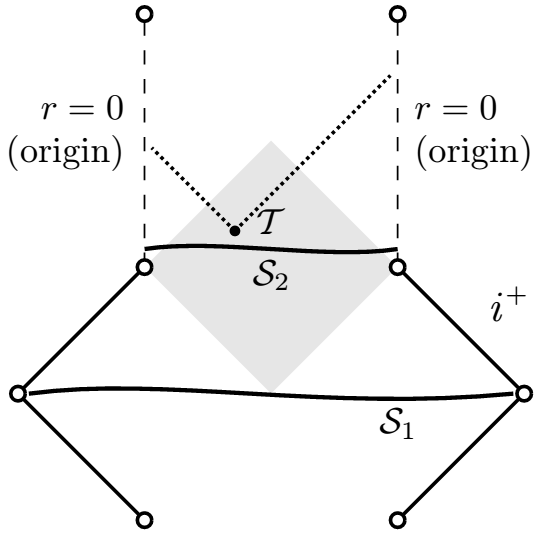
\includegraphics[width=0.35\textwidth]{bardeenDiagram}
	\caption{Estructura global de una porción del agujero negro de Bardeen. Imagen tomada de \cite{borde1994}.}
	\label{fig: bardeen diagram}
\end{figure}

Como se ha mencionado previamente, las propiedades globales, y en particular, la estructura causal de la métrica de Bardeen es similar a la de la métrica de Reissner Nordström, de ahí la similitud entre los diagramas de Penrose-Carter correspondientes a ambas métricas. Cada punto en el interior del espaciotiempo representado en la fig. \ref{fig: bardeen diagram} es una 2-esfera, las líneas sólidas y los círculos respresentan regiones en el infinito, y las líneas punteadas representan el origen ($r = 0$) del sistema de coordenadas esféricas (Las dos líneas eituqetadas con $r = 0$ representan dos "patches" diferentes de coordenadas). La región sombreada representa parte del interior del agujero negro, de tal forma que señales enviadas desde esa región no pueden escapar al infinito futuro tipo nulo $i^{+}$. Dado a que esa región, en particular, está dentro del horizonte de enventos del agujero, hay superficies atrapadas $\mathcal{T}$ en la misma. De acuerdo a Borde, el caráter regular de la métrica de Bardeen se debe a que, en la región señalada, es posible que los rayos de luz se ``envuelvan'' alrededor del universo universo, en otras palabras, aunque los sistemas de geodésicas nulas salientes o entrantes de $\mathcal{T}$ convergen, estas geodésicas convergen a puntos $r = 0$ de ``patches'' distintos. De hecho, la superficie atrapada $\mathcal{T}$ y su cono de luz futuro $E^{+}(\mathcal{T})$ yacen en el desarrolo de Cauchy futuro (OJO) de la superficie $\mathcal{S}_{2}$ y la singularidad en $r = 0$ se evita única y exclusivamente (OJO) debido a que $\mathcal{S}_{2}$ es compacta.\\

En otras palabras, las secciones espaciales de un agujero negro de Bardeen evolucionan (OJO) desde una región en la que no son compactas (por ejemplo, la superficie $\mathcal{S}_{1}$ de la fig. \ref{fig: bardeen diagram}), hacia una región donde son compactas, y por ende, el unvierso cambia su topología de abierto a cerrado. Estos razonamientos son formalizados por Bardeen mediante el siguiente teorema, en el cual se establece que dicho cambio de topología es necesario para la existencia de agujeros negros regulares que obedecen la condición de energía débil.\\

\begin{theorem}[Borde, 1996]
	\label{borde reg thm}
	Suponga que una espaciotiempo $\mathcal{M}$ satisface que
	
	\begin{enumerate}[i]
		\item contiene una superficie eventualmente futuramente atrapada $\mathcal{T}$,
		
		\item obedece la condición de convergencia nula,
		
		\item el cojunto de geodésicas nulas futuras es completo (OJO),
		
		\item su futuro causal es simple (OJO), con $E^{+}(X) \neq \emptyset,\ \forall X \subset \mathcal{M}$.
	\end{enumerate}
	
	Entonces hay una sección espacial compacta en el futuro de $\mathcal{T}$.
\end{theorem}

Una prueba (a simple vista, sencilla) de este teorema puede ser consultada en \cite{borde1996}. Es importante mencionar que, si bien no hay ninguna alución a un cambio de topología en el teorema, es usual que un espaciotiempo de agujero negro contenga una regiión en infinito (OJO) y, por ende, es de esperar que ``comience'' con una sección espacial no compacta $\mathcal{S}$ y por lo menos una superficie eventualmente futuramente atrapada en el futuro de la misma (OJO). En estos términos, el teorema de Borde muestra que, bajo condiciones muy generales, para que un agujero negro pueda ser regular se requiere que el espaciotiempo del cual hace parte desarrolle una sección espacial compacta en el futuro de $\mathcal{S}$, es decir, que la topología debe cambiar de abierta a cerrada. Una consecuencia inmediata de este cambio es que dicho espacio no puede ser globalmente hiperbólico.\\

¡OJO! Explicar cómo aplica el teorema para el caso de la métrica de Bardeen.\\

Para finalizar esta sección sobre la métrica de Bardeen es preciso mencionar que, si bien lo que hemos hecho hasta el momento es el primer paso para estudiar las estrellas de Planck, dichas estrellas son descritas por espaciotiempos que no son estáticos en absoluto. Por ende, es necesario desarrollar herramientas que permitan estudiar la evolución dinámica inminente de las susodichas estrellas. La forma en que se abordará espaciotiempos que varían con el tiempo será a través de la famosa métrica de Vaidya.

\subsection{Métrica de Vaidya}

La métrica de Vaidya \cite{padmanabhan} es una generalización de la métrica de Schwarzschild que puede ser interpretada como un espaciotiempo con una radiación saliente y esféricamente simétrica de partículas sin masa.\\

Esta métrica puede ser hallada a partir de la de Schwarzschild 

\begin{equation}
ds^2 = -\left( 1 - \frac{2m}{r} \right) + \left( 1 - \frac{2m}{r} \right)^{-1}dr^2 + r^2d\Omega^2,
\end{equation}
y para ello es necesario pasar a coordenadas de Eddington-Finkelstein, en las que la coordenada temporal $t$ es reemplazada por una nueva coordenada $u$ que satisface

\begin{equation}
dt = du + \frac{dr}{(1 - 2m/r)}.
\end{equation}

Para la interpretación física de esta nueva coordenada, note que $u = cte$ corresponde a curvas que satisfacen la ecuación $dr/dt = +\left( 1 -2m/r \right)$. Las líneas radiales nulas en el espaciotiempo de Schwarzschild corresponden a curvas con $d\theta = d\phi = ds = 0$ y en términos de $r$ y $t$ satisfacen $(dr/dt)^2 = \left( 1 -2m/r \right)^2$. La raíz positiva de esta ecuación representa líneas de tipo nulo dirigidas radialmente hacia afuera (la raíz negativa, a rayos dirigidos radialmente hacia adentro).\\

Con dicha transformación, el elemento de línea se convierte en 

\begin{equation}
\label{schw-tortoise}
ds^2 = - \left(1- \frac{2m}{r}\right)du^2 - 2dudr + r^2d\Omega^2.
\end{equation}

Dado que nos interesa llegar a una métrica debida a fotones dirigidos radialmente hacia afuera, podemos considerar una generalización de \eqref{schw-tortoise} a una métrica dinámica en la que m varía respecto a la nueva coordenada temporal $u$, esto es, $m = m(u)$. Por ende Teniendo en cuenta lo anterior, el tensor energía-momento que genera la métrica \eqref{schw-tortoise} tiene como única componente distinta de cero $T_{uu} = -(m'/4 \pi r^2)$, con $m' = dm(u)/du$. Esto es exactamente igual al tensor que se obtendría para un rayo de fotones moviéndose radialmente hacia afuera con cuadrimomento $k_{a} = \nabla_{a}u$. El EMT en este caso es $T^{ab} = -(m'/4 \pi r^2)k^{a}k^{b}$. Dado lo anterior, podemos interpretar la métrica de Vaidya como debida a una fuente esféricamente simétrica que pierde masa al emitir fotones en la dirección radial.\\

Con respecto a las condiciones de energía, es claro que por la forma del EMT para la métrica de Vaidya, la única condición que vale la pena estudiar es WEC, la cual requiere $T_{uu} \geq 0$ y en términos de r requiere que $m'(u)\leq 0 $. Esta última condición coincide precisamente con la interpretación previamente mencionada sobre que la métrica de Vaidya describe una estrella pierde masa conforme pasa el tiempo mediante la emisión de radiación en forma de fotones.\\

Ahora bien, a parte de la presencia de radiación, la métrica de Vaidya posee una característica fundamental que la diferencia radicalmente de la métrica de Schwarzschild, y esto es el tipo de superficie (horizonte) en $r = 2m(u)$. En el espacioteimpo de Schwarzschild, $r = 2m$ representa una superficie de tipo nulo que denota el conocido horizonte de eventos. Por su parte, a continuación se verá que en el espaciotiempo de Vaidya la superficie $r = 2m(u)$ es de tipo espacio y por ende no puede ser asociada a un horizonte de eventos. De hecho, esta superficie conforma lo que usualmente es denominado en la literatura \cite{blau,griffiths2009,wald2010} como horizonte aparente.\\


Un horizonte aparente se define técnicamente como una hipersuperficie que separa las regiones que poseen superficies atrapadas de las regiones que no contienen este tipo de superficies. No obstante, en aras de dar una definción matemáticamente más concreta de horizontes aparentes es necesario formalizar matmáticamente la definición de hipersuperficies nulas y definir el concepto de divergencia de campos vectoriales.\\

Como es sabido, una hipersuperficie es una subvariedad $\Sigma$ n-dimensional de una variedad $M$ n+1-dimensional \cite{blau}. Una descripción particularmente útil para estudiar la geometría de estas subvariedades se da a través de los embebimientos $\Phi: \Sigma \to M$. Si $\Sigma$ es equipado con coordenadas $y^\alpha$ y $M$ con coordenadas $x^\alpha$, un embebimiento $\Phi$ está dado explícitamente al especificar el punto en $M$ con coordenadas $x^\alpha$ que corresponde a un punto en $\Sigma$ con coordenadas $y^\alpha$, en otras palabras, un embebimiento está dado por las ecuaciones paramétricas 
\begin{equation*}
x^\alpha = x^\alpha(y^\alpha).
\end{equation*}

Hay dos condiciones que deben ser satisfechas para que un mapa $\Phi$ sea un embebimiento, a saber
\begin{itemize}
	\item $\Phi$ debe ser inyectivo.
	\item El jacobiano de $\Phi$, es decir, la matriz $(n+1)\times n$
	\begin{equation*}
	E^{\alpha}_{a} = \frac{\partial x^\alpha}{\partial y^\alpha},
	\end{equation*}
	
	tiene rango maximal n.
\end{itemize}

Dado que los vectores $E^{\alpha}_{a}$ son linealmente independientes y tangentes a la imagen de $\Sigma$ en $M$, los vectores normales a $\Sigma$ (es decir, orthonormales a $\Sigma$) están caracterizados por 
\begin{equation*}
g_{\alpha \beta}E^{\alpha}_{a}\xi^{\alpha} = E^{\alpha}_{a}\xi_{\beta} = 0,
\end{equation*}

con $g_{\alpha \beta}$ la métrica de $M$. Es importante notar que si $\xi^{\alpha}$ es un vector normal, entonces $f\xi^{\alpha}$ también es normal a $\Sigma$ para cualquier función escalar $f$ que es distinta de cero en $\Sigma$.\\

Teniendo en cuenta lo anterior, los vectores normales a $\Sigma$ permiten establecer la siguiente caracterización de hipersuperficies
\begin{align*}
\Sigma\ es\ tipo\  
\begin{cases}
\ espacio\ & si\ \xi^{\alpha}\xi_{\alpha}<0,\\
\ tiempo\ & si\ \xi^{\alpha}\xi_{\alpha}>0,\\
\ nulo\ & si\ \xi^{\alpha}\xi_{\alpha}=0.\\
\end{cases}
\end{align*}

Cuando $\Sigma$ no es nula, la libertad en la elección de $f$ puede ser usada para normalizar el vector normal a un vector normal de longitud unitaria $\pm 1$. Esta codición de normalización determina el vector normal unitario $N^{\alpha}$ de forma única salvo una elección de signo, esto es
\begin{align*}
N^{\alpha} = \frac{\xi^{\alpha}}{|\xi^{\alpha}\xi_{\alpha}|^{1/2}} \Rightarrow N^{\alpha}N_{\alpha} =\ 
\begin{cases}
\ -1 & \ si\ \Sigma\ es\ tipo\ espacio,\\
\ +1 & \ si\ \Sigma\ es\ tipo\ tiempo.\\
\end{cases}
\end{align*}

Evidentemente, esta normalización es imposible para las hipersuperficies tipo nulo. No obstante, una elección natural y conveniente de un vector normal a la hipersuperficie es 
\begin{equation*}
l_\alpha = -\partial_\alpha S,
\end{equation*}

donde el signo ha sido escogido de tal forma que $l^\alpha$ está orientado hacia el futuro para una fución real-valuada $S$ que aumenta hacia el futuro y en términos de la cual la hipersuperficie $\Sigma$ se define como
\begin{equation*}
\Sigma = \lbrace x \in M:\ S(x) = 0 \rbrace.
\end{equation*}

De esta forma, los demás vectores normales a $\Sigma$ son de la forma
\begin{equation*}
\xi^\alpha = fl^\alpha,
\end{equation*}

para alguna función $f$ que no se anula sobre $\Sigma$.\\

Ahora bien, con las herramientas anteriores es posible definir la métrica inducida $h_{ab}$ en una hipersuperficie (nula), y la utilidad de $h_{ab}$ recae en que a partir de la misma, la identificación del tipo al cual pertenece una hipersuperfcie dada es automático, permitiéndonos diferenciar fácilmente entre horizontes ade eventos y horizontes aparentes.\\

Dado que en general las geodésicas nulas que son los generadores de una hipersuperficie nula están naturalmente asociados a dicha hipersuperficie, es conveniente adaptar las coordenadas $y^\alpha$ en $\Sigma$ a $l^\alpha$ al escoger las coordenadas de tal forma que 
\begin{equation*}
y^\alpha = (v = \lambda, y^k),
\end{equation*}

donde $\lambda$ es el parámetro (no necesariamente afín) a lo largo de las geodésicas y $y^k$ coresponde a las coordenadas espaciales que denotan las geodésicas nulas individuales. En estas coordenadas, los vectores tangentes $E_\alpha$ a la hipersuperficie nula están dados por
\begin{equation*}
E^{\alpha}_{v} = \frac{\partial x^\alpha}{\partial \lambda} = l^\alpha \hspace{.5cm}, \hspace{.5cm} E^{\alpha}_{k} =\frac{\partial x^\alpha}{\partial y^k},
\end{equation*}

y por ende la métrica inducida
\begin{equation*}
h_{ab} = g_{\alpha \beta} E^{\alpha}_{a} E^{\alpha}_{b},
\end{equation*}

tiene los componentes 

\begin{equation*}
h_{vv} = g_{\alpha \beta} l^\alpha l^\beta = 0 \hspace{.5cm},\hspace{.5cm} h_{vk} = g_{\alpha \beta} l^\alpha E^{\beta}_{k} = 0, \hspace{.5cm},\hspace{.5cm} h_{km} \equiv s_{km} = g_{\alpha \beta} E^{\alpha}_{k} E^{\beta}_{m},
\end{equation*}

donde $h_{vk} = 0$ se sigue puesto que por construcción los vectores $E^{\alpha}_{k}$ son tangentes a la superficie mientras que por definición $l^\alpha$ es normal a la hipersuperficie y en particular normal a los vectores tangentes a la misma. \\

Dado lo anterior, la métrica es degenerada (lo cual es característico para las hipersuperficies nulas) y el elemento de línea toma la forma
\begin{equation*}
ds^2|_{\substack{\Sigma}} = s_{km}dy^k dy^m = g_{\alpha \beta} E^{\alpha}_{k} E^{\beta}_{m} dy^k dy^m.
\end{equation*}

Es importante notar que esta forma de la métrica es independiente de si el parámetro $\lambda$ es o no el parámetro afín de las geodésicas nulas, puesto que la escogencia de este parámetro puede ser tenida en cuenta al cambiar $l^\alpha \to \xi^\alpha = fl^\alpha$ para alguna ellección apropiada de $f$, de tal forma que siempre se tiene $h_{vv} = h_{vk} = 0$.

Con la finalidad de acercarnos a la definción de divergencia de un campo vectorial, la última herramienta requerida para la diferenciación entre horizontes de eventos y horizontes aparentes es el vector auxiliar $n$ que satisface las siguientes propiedades
\begin{equation*}
n_\alpha n^\alpha = n_\alpha n^\alpha \hspace{.5cm},\hspace{.5cm} n_\alpha E^{\alpha}_{k} =  n_\alpha E^{\alpha}_{k} = 0 \hspace{.5cm},\hspace{.5cm} n_\alpha l^\alpha = -1,
\end{equation*}

que corresponde a un vector normal en $\Sigma$ pero no tangente, que es linealmente independiente tanto a $E^{\alpha}_{k}$ como a $l^\alpha$.

\section{\label{planck stars section} Métrica de Hayward}

Teniendo todas las herramientas estudiadas en las seccioes anteriores, es posible comenzar a estudiar el tema de interés para este trabajo, a saber, la métrica correspondiente a las estrellas de Planck.

\subsection{Métrica de Hayward estática}

Si bien es posible encontrar métricas como la de Bardeen, es decir, esféricamente simétricas, estáticas, asintóticamente planas, con centros regulares, cuyos EMT es físicamente razonable, en particular que satisface la WEC. No obstante, dichos espaciotiempos típicamente soy considerados como no-físicos en tanto que poseen horizontes de Cauchy (OJO). No obstante, si consideramos la evaporación de uno de esos agujeros negros, el horizonte de cauchy pasa a user tan real como el horizonte de eventos.  Precisamente, las estrellas de Planck son descritas por métricas regulares dno estáticas (dinámicas) que satisfacen todas las propiedades anteriormente mencionadas, y que además poseen la característica adicional de incluir correcciones de teoría cuántica de campos en relatividad general.\\

Con el fin de entender paulatinamente el concepto de estrella de Planck, es preciso dividir su estudio entre la parte estática y la parte dinámica. La parte estática es descrita por la métrica de Hayward, la cual está dada por 

\begin{equation}
\label{hayward metric}
ds^2 = -\left( 1 - \frac{mr^2}{r^3 + 2ml^2} \right) dt^2 + \left( 1 - \frac{mr^2}{r^3 + 2ml^2} \right)^{-1} dr^2 + r^2d\Omega ^2,
\end{equation}

donde $m$ y $l$ son parámetros cuya interpretación física se explicará más adelante. Claramente, para esta métrica tenemos que

\begin{equation}
\label{hayward mass}
m(r) =  \frac{mr^3}{r^3 + 2ml^2}.
\end{equation}

Por ende, la métrica de Hayward satisface inmediatamente la WEC en tanto que 

\begin{equation}
\begin{aligned}
\frac{1}{r^2}\frac{dm(r)}{dr} &= \frac{12 l^2 m^2}{\left(2 l^2 m+r^3\right)^2},\\
\frac{2}{r}\frac{dm(r)}{dr} &= \frac{24 l^2 m^2 r}{\left(2 l^2 m+r^3\right)^2},\\
\frac{d^2m(r)}{dr^2} &= \frac{48 m^2 \left(l^4 m r-l^2 r^4\right)}{\left(2 l^2 m+r^3\right)^3}.
\end{aligned}
\end{equation}

Como en el caso de Bardeen, la métrica de Hayward describe un espaciotiempo regular puesto que, por un lado, 

\begin{equation}
f_{hayward}(r) \underset{r \to 0}{\sim} 1 - \frac{r^2}{l^2} + \mathcal{O}(r^5),
\end{equation}

es decir, es de Sitter en la vecindad de $r =0$, y por otro, sus invariantes de curvatura

\begin{equation}
\label{hayward scalars}
\begin{gathered}
R = \frac{24 l^2 m^2 \left(4 l^2 m-r^3\right)}{\left(2 l^2 m+r^3\right)^3},\\
R_{\mu \nu}R^{\mu \nu} = \frac{288 m^4 \left(8 l^8 m^2-4 l^6 m r^3+5 l^4 r^6\right)}{\left(2 l^2 m+r^3\right)^6},\\
R_{\mu \nu \sigma \rho}R^{\mu \nu \sigma \rho} = \frac{48 m^2 \left(32 l^8 m^4-16 l^6 m^3 r^3+72 l^4 m^2 r^6-8 l^2 m r^9+r^{12}\right)}{\left(2 l^2 m+r^3\right)^6},
\end{gathered}
\end{equation}

permanecen finitos en todo el espaciotiempo.\\

Ahora bien, al analizar los ceros de $f_{hayward}(r)$ revela una masa crítica de $m_{*} = (3\sqrt{3}/4)l$ y un radio crítico de $r = \sqrt{3}l$. Dado lo anterior, si $m < m_{*}$, la métrica \ref{hayward metric} describe un espaciotiempo regular con la misma estructura causal que cualquier espaciotiempo plano; si $m = m_{*}$ tenemos un agujero negro regular con un único horizonte de eventos degenerado; y si $m > m_{*}$ tenemos un agujero negro con dos horizontes de eventos. Esto se ve reflejado en la fig. \ref{fig: fhayward analysis}. 

\begin{figure}[h!]
	\centering
	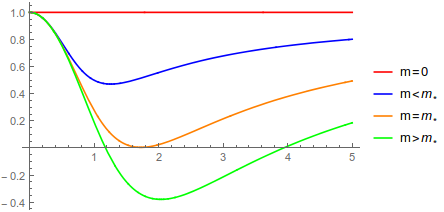
\includegraphics[width=0.75\textwidth]{fhaywardAnalysis}
	\caption{Posibles casos de agujeros negros para la métrica de Hayward con para un valor fijo del parámetro $l$ y diferentes valores del parámetro $m$. La estructura causal de este espaciotiempo es similar a la de Reissner Norström.}
	\label{fig: fhayward analysis}
\end{figure}

Evidentemente, la pregunta natural con respecto a las anteriores consideraciónes es cuál es la fuente física que da origen a esta métrica. Para contestarla, note que 

\begin{equation}
f_{hayward}(r) \underset{r \to \infty}{\sim} 1 - \frac{2m}{r} + \frac{4l^2m^2}{r^4} + \mathcal{O}(r^{-5}),
\end{equation}

luego, al igual que en el caso de Bardeen, podemos interpretar el parámetro $m$ como la masa de la distribución que genera el elemento de línea \eqref{hayward metric}. No obstante, dada la presencia del término $r^{-4}$, es imposible interpretar el parámetro $l$ en términos de una carga coulombiana. De hecho, Hayward plantea que $l$ da aproximadamente la escala de longitud debajo de la cual los efectos de cuánticos en gravedad comienzan a ser dominantes, razón por la cual es de esperar que $l$ sea la longitud de Planck o del mismo orden de magnitud, aunque longitudes mayores no son excluídas. Cabe mencionar que sería interesante hallar una interpretación física para el parámetro $l$ tal como se mostró para el parámetro $g$ en el caso de Bardeen, es decir, hallando una fuente de electrodinámica no-lineal para la función de masa \eqref{hayward mass}, y por ende, para el elemento de línea \eqref{hayward metric}. Si hay suficiente tiempo, dicha interpretación se colocará en la sección de anexos.\\


\subsection{Métrica de Hayward dinámica}

Para la parte dinámica de las estrellas de Planck es preciso considerar la coordenada avanzada de Eddignton-Finkelstein entrantes, las cuales se obtienen a partir de

\begin{equation}
dt = dv - \frac{dr}{(1 - 2m/r)}.
\end{equation}

En términos de la nueva coordenada, el elemento de línea \eqref{hayward metric} se transforma en 

\begin{equation}
\label{hayward-tortoise}
ds^2 = -\left( 1 - \frac{mr^2}{r^3 + 2ml^2} \right) dv^2 + 2dvdr + r^2d\Omega ^2,
\end{equation}

y al generalizar la función de masa a $m = m(v)$ tenemos que el EMT asociado a \eqref{hayward-tortoise} es

\begin{equation}
\begin{aligned}
T_{t}^{\ t} &= T_{r}^{\ r} = -\frac{12 l^2 m^2}{\left(2 l^2 m+r^3\right)^2}, \\
T_{\theta}^{\ \theta} &= T_{\phi}^{\ \phi} = -\frac{24 l^2 m^2 \left(l^2 m-r^3\right)}{\left(2 l^2 m+r^3\right)^3},\\
T_{v}^{\ r} &= \frac{2r^4m'}{(r^3 + 2l^2m)^2},
\end{aligned}
\end{equation}

donde $m' = dm/dv$. Las componentes $T_{t}^{\ t}$, $T_{r}^{\ r}$, $T_{\theta}^{\ \theta}$, $T_{\phi}^{\ \phi}$ son iguales a los de la métrica de Hayward estática, la única novedad es la componente $T_{v}^{\ r}$, la cual describe puramente la radiación entrante que fue incorporada al modelo al considerar $m = m(v)$.\\

¡OJO! 1/8$\pi$ en los EMT

\section{Métrica de Hayward modificada}

Con respecto a lo mencionado sobre la escala de Planck, estudios posteriores al artículo de Hayward (véase \cite{lorenzo}) han hecho explícito el hecho de que la presencia del paŕametro de longitud $l$ en la métrica de Hayward necesariamente refleja la inclusión de correcciones efectivas de teoría cuántica de campos en relatividad general. Al respecto, De Lorenzo \emph{et al.} plantean que, para que las métricas que describen espaciotiempos regulares a partir de modificaciones de la métrica de Schwarzschild sean físicamente plausibles, se requieren dos condiciones: que dichas métricas incorporen las correcciones efectivas de teoría cuántica  de campos al potencial Newtoniano, y una dilatación temporal no trivial entre un observador en $r \to \infty$ y un observador en $r = 0$. Precisamente, esta sección se encarga de estudiar con más detalle estos aspectos.\\

De acuerdo a De lorenzo \emph{et al.}, la mayoría de las métricas correspondientes a modelos de agujeros negros regulares poseen dos características que carecen de sentido físico, a saber, que un reloj en el centro regular no presenta ningún retraso con respecto a un reloj en el infinito, y que no reroducen las correcciones efectivas de toería cuańtica de campos al potencial Newtoniano \cite{lorenzo}. Por estos motivos, los autores proponen una modificación a la métrica de interés, en este caso la de Hayward, que corrige estos ``defectos'' de dicha métrica.\\

La corrección efectiva de teoría cuántica de campos al potencial Newtoniano es

\begin{equation}
\label{newF}
\Phi (r) = -\frac{M}{r} \left( 1 + \beta \frac{l_{p}^2}{r^2} \right) + \mathcal{O}(r^{-4}),
\end{equation}

donde $l_{p}$ en la longitud de Planck.\\

La métrica de Hayward modificada está dada por 
\begin{equation}
\label{reg-schF}
ds^2 = -G(r)F(r) dt^2 + \frac{1}{F(r)} dr^2 + r^2d\Omega ^2
\end{equation}

donde

\begin{equation}
\label{mod-hay-f}
F(r) = 1 - \frac{Mr^2}{r^3 + 2ML^2}
\end{equation}

\begin{equation}
\label{mod-hay-g}
G(r) = 1 - \frac{\beta M \alpha}{\alpha r^3 + \beta M}
\end{equation}

\section{\label{conclusions} Conclusiones}

\section{\label{annex} Anexos}

¡OJO! Correcciones cuánticas\\

\newpage
\nocite{*}
\bibliographystyle{unsrt}
\bibliography{Biblio}


\end{document} 